\documentclass[a4paper,12pt]{article}
\usepackage[brazil]{babel}
\usepackage[utf8]{inputenc}
\usepackage[T1]{fontenc}
\usepackage{geometry}
\usepackage{setspace}
\usepackage{titlesec}
\usepackage{hyperref}
\usepackage{graphicx}
\usepackage{caption}
\usepackage{subcaption}
\usepackage{fancyhdr}
\usepackage{xcolor}
\usepackage{pdfpages}

\input{commands.tex}

\hypersetup{
    colorlinks=true,% make the links colored
    linkcolor=blue
}

\usepackage{setspace}
\addbibresource{bibliography.bib}

\newcommand{\printingbibliography}{%

    \pagestyle{myheadings}
    \markright{}
    \sloppy
    \printbibliography[heading=bibintoc, % add to table of contents
                   title=Refer\^encias % Chapter name
                  ]
    \fussy%
}
\PassOptionsToPackage{table}{xcolor}
\renewcommand{\baselinestretch}{1.5}

\pagestyle{fancy}
\fancyhf{}
\renewcommand{\headrulewidth}{0pt}
\fancyhead[R]{\thepage}

\geometry{a4paper,top=30mm,bottom=20mm,left=30mm,right=20mm}

\titleformat*{\section}{\bfseries\large}
\titleformat*{\subsection}{\bfseries\normalsize}

\title{}
\author{Andr\'e V. Silva}
\date{\today}

\begin{document}

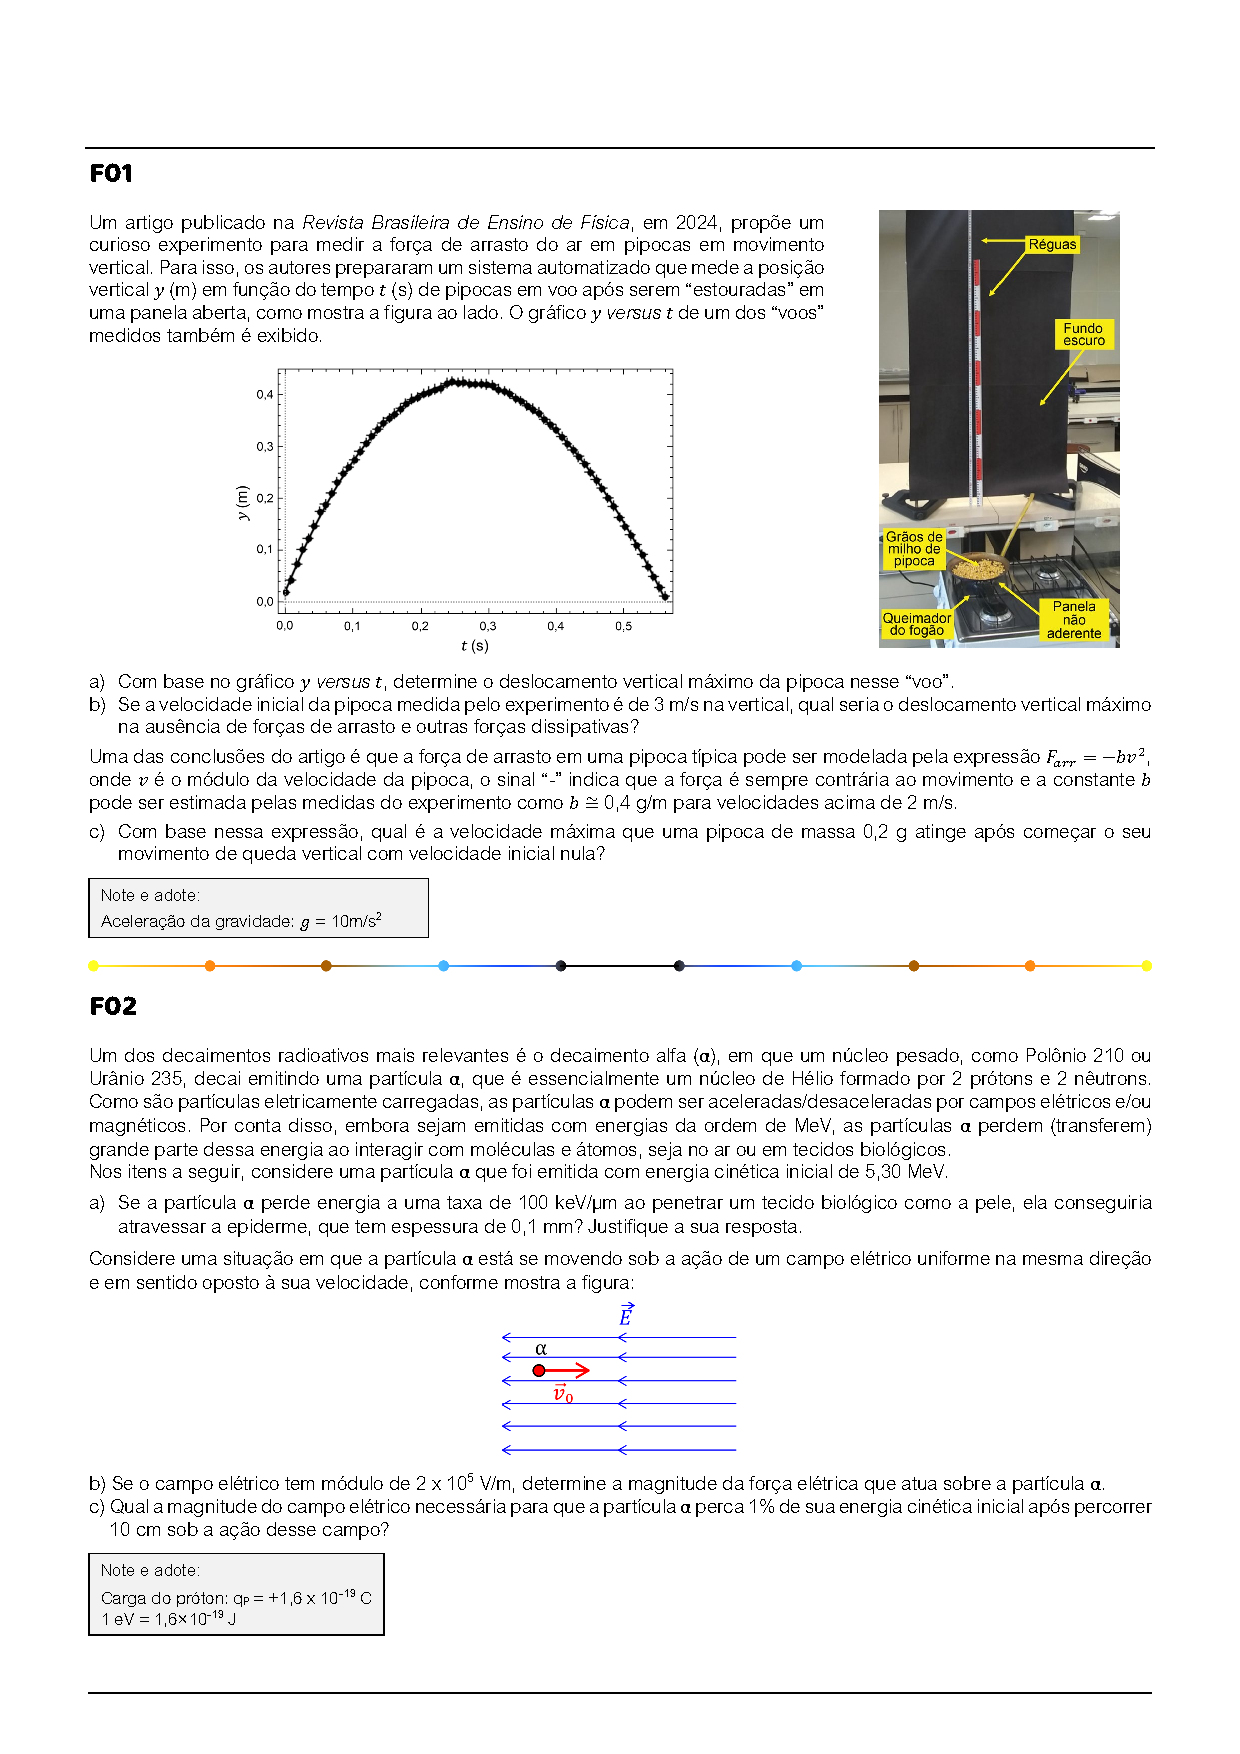
\includepdf[pages=-]{pg_0002.pdf}

\maketitle

\begin{figure}[ht]
\centering
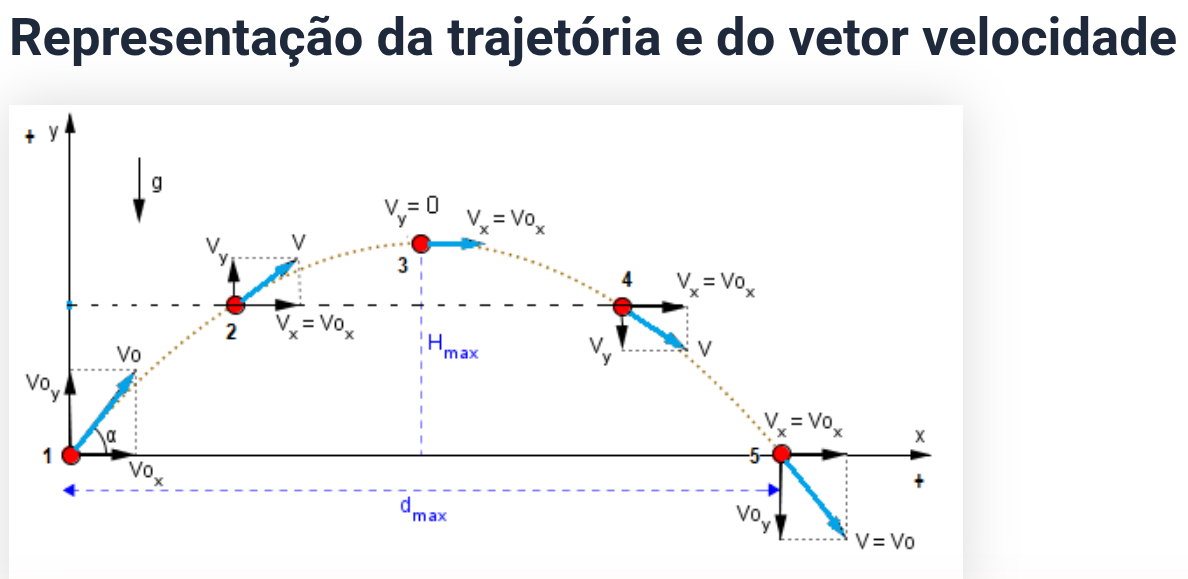
\includegraphics[width=0.9\textwidth]{images/momentoobliquo.png}
\end{figure}


\section*{Introdução Teórica}

O movimento de um objeto lançado verticalmente na presença da gravidade é um problema clássico da Mecânica. Em muitas situações ideais, despreza-se a resistência do ar e considera-se apenas a força peso atuando sobre o corpo. Entretanto, em sistemas reais, especialmente quando os objetos possuem baixa massa e grande área superficial, como é o caso de uma pipoca em voo, os efeitos da resistência do ar tornam-se relevantes e modificam significativamente o movimento.

\subsection*{Lançamento vertical sob ação da gravidade}

Quando um objeto é lançado verticalmente com velocidade inicial \(v_0\), sob a ação exclusiva da gravidade, ele realiza um movimento uniformemente variado. A aceleração é constante e igual à aceleração da gravidade \(g\), dirigida para baixo.

As equações cinemáticas que descrevem esse movimento são:

\[
v_{y}(t)=v_{0y} - gt
\]

\[
y(t)=y_0 + v_{0y} t - \frac{1}{2}gt^2
\]

onde:

\begin{itemize}
\item \(y(t)\) é a posição vertical em função do tempo,
\item \(v(t)\) é a velocidade instantânea,
\item \(y_0\) é a posição inicial,
\item \(v_0\) é a velocidade inicial,
\item \(g\) é a aceleração da gravidade.
\end{itemize}

Durante a subida do objeto, sua velocidade diminui gradualmente até se anular no ponto mais alto da trajetória. Nesse ponto ocorre o deslocamento vertical máximo.

A altura máxima pode ser determinada a partir da equação de Torricelli:

\[
v_{y}^2 = v_{0y}^2 - 2g(y - y_0)
\]

No ponto mais alto, \(v=0\), resultando em:

\[
h_{max} = \frac{v_{0y}^2}{2g}
\]

Essa expressão fornece o deslocamento vertical máximo quando não existem forças dissipativas atuando no sistema.

\subsection*{Influência da resistência do ar}

Na prática, o movimento de um corpo que se desloca em um fluido sofre a ação de uma força de resistência, conhecida como força de arrasto. Essa força depende da velocidade do objeto e atua sempre em sentido oposto ao movimento.

Para diversos regimes de velocidade, especialmente em objetos leves movendo-se no ar, uma aproximação comum consiste em modelar a força de arrasto como proporcional ao quadrado da velocidade:

\[
F_{arr} = -b v^2
\]

onde:

\begin{itemize}
\item \(b\) é uma constante que depende das propriedades do fluido, da forma e da área do objeto,
\item \(v\) é o módulo da velocidade do corpo,
\item o sinal negativo indica que a força atua no sentido contrário ao movimento.
\end{itemize}

Assim, a equação dinâmica que descreve o movimento passa a ser obtida a partir da Segunda Lei de Newton:

\[
\sum F = ma
\]

Durante a queda vertical, duas forças principais atuam sobre o corpo:

\begin{itemize}
\item a força peso \(P = mg\), dirigida para baixo;
\item a força de arrasto \(F_{arr}\), dirigida para cima quando o corpo se move para baixo.
\end{itemize}

A equação de movimento pode então ser escrita como:

\[
mg - bv^2 = ma
\]

\subsection*{Velocidade terminal}

À medida que o corpo cai, sua velocidade aumenta e, consequentemente, o módulo da força de arrasto também cresce. Em determinado momento, essa força torna-se suficientemente grande para equilibrar a força peso.

Quando isso ocorre, a força resultante sobre o corpo torna-se nula:

\[
mg = bv^2
\]

Nessa condição, a aceleração desaparece e o corpo passa a mover-se com velocidade constante. Essa velocidade é denominada \textbf{velocidade terminal}.

Resolvendo a equação para \(v\), obtém-se:

\[
v_t = \sqrt{\frac{mg}{b}}
\]

Esse resultado mostra que a velocidade terminal depende da massa do objeto, da aceleração da gravidade e da constante de arrasto associada ao meio e à geometria do corpo.

\subsection*{Análise experimental do movimento}

Uma forma eficiente de estudar esse tipo de movimento consiste em registrar experimentalmente a posição do objeto ao longo do tempo, obtendo um gráfico \(y(t)\). A análise desse gráfico permite determinar grandezas importantes como:

\begin{itemize}
\item o deslocamento vertical máximo,
\item o tempo de subida e descida,
\item a influência das forças dissipativas no movimento.
\end{itemize}

Experimentos desse tipo são particularmente interessantes em objetos leves, como pipocas, pois a interação com o ar é significativa e permite observar claramente os efeitos da resistência do fluido.

\section*{F1 - Resolu\c{c}\~ao}

\textbf{\textcolor{blue}{\Large Quest\~ao - Movimento vertical com resist\^encia do ar}}

\subsection*{Resolu\c{c}\~ao}

O problema descreve o movimento vertical de uma pipoca após ser lançada para cima quando o grão estoura. O experimento mede a posição vertical \(y\) em função do tempo \(t\), permitindo analisar o movimento por meio do gráfico apresentado.

\subsubsection*{(a) Determinação do deslocamento vertical máximo a partir do gráfico}

O deslocamento vertical máximo corresponde ao ponto mais alto da trajetória da pipoca. No gráfico \(y \times t\), esse valor corresponde ao vértice da curva.

Observando o gráfico:

\begin{itemize}
\item o eixo vertical representa a posição \(y\) em metros;
\item os valores variam aproximadamente entre \(0\) e \(0{,}45\,\text{m}\);
\item o ponto máximo da curva ocorre aproximadamente em \(y \approx 0{,}42\,\text{m}\).
\end{itemize}

Portanto, o deslocamento vertical máximo medido experimentalmente é aproximadamente

\[
y_{\max} \approx 0{,}42\,\text{m}.
\]

Esse valor é obtido diretamente da análise do gráfico experimental.

\subsubsection*{(b) Deslocamento máximo na ausência de forças dissipativas}

Agora considera-se a situação ideal em que apenas a força peso atua sobre a pipoca, ou seja, despreza-se a resistência do ar.

Nesse caso, o movimento vertical é uniformemente variado e podemos utilizar a equação de Torricelli:

\[
v_{y}^2 = v_{0y}^2 - 2g(y - y_0)
\]

No ponto mais alto da trajetória, a velocidade é nula:

\[
v_{y}=0
\]

Logo,

\[
0 = v_{0y}^2 - 2g h_{\max}
\]

onde \(h_{\max} = y - y_0\) representa o deslocamento vertical máximo.

Isolando \(h_{\max}\):

\[
h_{\max} = \frac{v_{0y}^2}{2g}
\]

Substituindo os valores fornecidos:

\[
v_0 = 3\,\text{m/s}
\]

\[
g = 10\,\text{m/s}^2
\]

temos

\[
h_{\max} = \frac{(3)^2}{2 \cdot 10}
\]

\[
h_{\max} = \frac{9}{20}
\]

\[
h_{\max} = 0{,}45\,\text{m}
\]

Portanto, na ausência de forças dissipativas, o deslocamento vertical máximo seria

\[
h_{\max} = 0{,}45\,\text{m}.
\]

Esse valor é ligeiramente maior do que o valor experimental obtido no item anterior, o que evidencia o efeito da resistência do ar no experimento.

\subsubsection*{(c) Velocidade máxima durante a queda (velocidade terminal)}

O problema informa que a força de arrasto pode ser modelada pela expressão

\[
F_{arr} = -b v^2
\]

onde:

\begin{itemize}
\item \(b\) é uma constante experimental;
\item \(v\) é o módulo da velocidade;
\item o sinal negativo indica que a força é contrária ao movimento.
\end{itemize}

Durante a queda vertical, atuam duas forças principais sobre a pipoca:

\begin{itemize}
\item a força peso \(P = mg\), dirigida para baixo;
\item a força de arrasto \(F_{arr}\), dirigida para cima.
\end{itemize}

A velocidade máxima ocorre quando a aceleração se torna nula, isto é, quando a força resultante é zero. Essa velocidade é chamada de \textbf{velocidade terminal}.

Aplicando a segunda lei de Newton:

\[
\sum F = ma
\]

Na condição de velocidade terminal:

\[
a=0
\]

Logo,

\[
mg - b v^2 = 0
\]

ou

\[
mg = b v^2
\]

Isolando \(v\):

\[
v = \sqrt{\frac{mg}{b}}
\]

\subsubsection*{Substituição dos valores}

A massa da pipoca é

\[
m = 0{,}2\,g
\]

Convertendo para unidades do SI:

\[
m = 0{,}2 \times 10^{-3}\,\text{kg}
\]

\[
m = 2 \times 10^{-4}\,\text{kg}
\]

A constante de arrasto fornecida é

\[
b = 0{,}4\,g/m
\]

Convertendo:

\[
b = 0{,}4 \times 10^{-3}\,\text{kg/m}
\]

\[
b = 4 \times 10^{-4}\,\text{kg/m}
\]

Substituindo na expressão da velocidade terminal:

\[
v = \sqrt{\frac{(2 \times 10^{-4})(10)}{4 \times 10^{-4}}}
\]

\[
v = \sqrt{\frac{20}{4}}
\]

\[
v = \sqrt{5}
\]

\[
v \approx 2{,}24\,\text{m/s}
\]

Portanto, a velocidade máxima que a pipoca atinge durante a queda é aproximadamente

\[
v_{\max} \approx 2{,}2\,\text{m/s}.
\]

\subsubsection*{Conclusão}

\begin{itemize}
\item O deslocamento vertical máximo observado no experimento é aproximadamente \(0{,}42\,\text{m}\).
\item Na ausência de resistência do ar, a altura máxima seria \(0{,}45\,\text{m}\).
\item A velocidade máxima durante a queda, determinada pelo equilíbrio entre peso e arrasto, é aproximadamente \(2{,}2\,\text{m/s}\).
\end{itemize}

Esses resultados mostram claramente o efeito da resistência do ar no movimento de objetos leves, como uma pipoca em voo.



%%%%%%%% Bibliography 
% Os comandos para incluir as referências bibliográficas
\printingbibliography

\end{document}
